%! Author = drakanoy
%! Date = 10.09.2024

% Preamble
\documentclass[12pt]{article}

% Packages
\usepackage[utf8]{inputenc}
\usepackage[T2A]{fontenc}
\usepackage[english, russian]{babel}
\usepackage[a4paper, includefoot, left=1.5cm, right=1.5cm, top=1cm, bottom=1.5cm, headsep=1cm, footskip=1cm]{geometry}
\usepackage{makecell}
\usepackage{amsmath}
\usepackage{graphicx}
\usepackage{enumitem}
\usepackage{svg}
\usepackage{multirow}
\usepackage{hyperref}
\usepackage{mathtools}
\usepackage{amssymb}
\usepackage{textcomp}

% Document
\begin{document}
\begin{large}
\begin{center}
\LARGE \textbf{Домашняя работа}
\par
\LARGE \textbf{Кононов Александр Михайлович}
\par
    \textbf{30.11.2024}
\end{center}
\par Условие:
\par
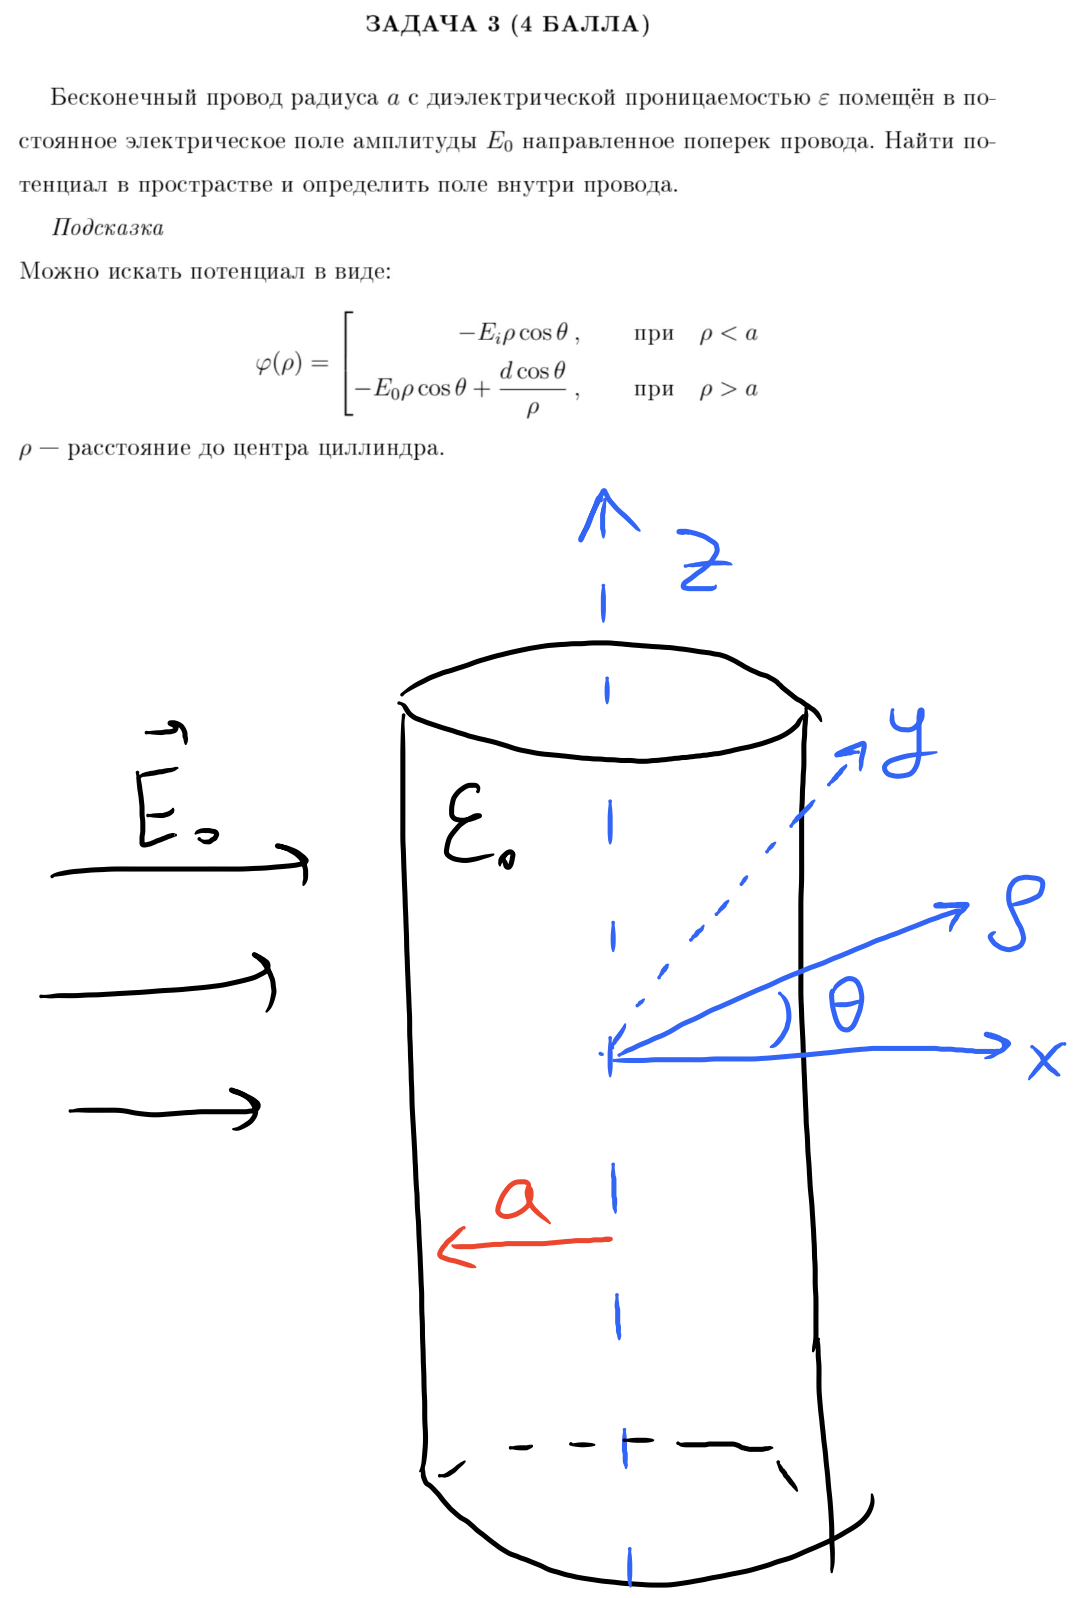
\includegraphics[width=1\textwidth]{photo.png}
%\begin{center}
%\underline{Рисунок 1}:
%\end{center}
\par Решение:
\par
\par
%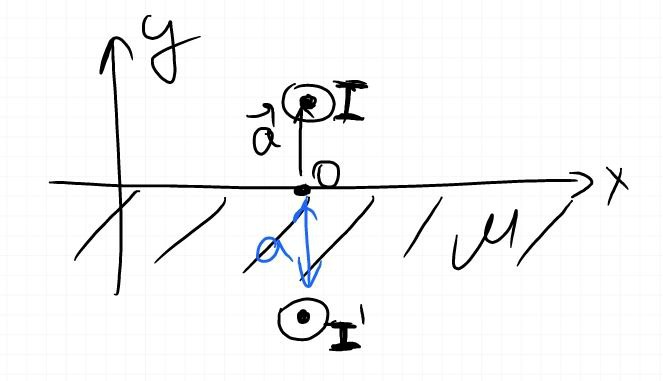
\includegraphics[width=1\textwidth]{photo_1.jpg}
%\par
\begin{center}
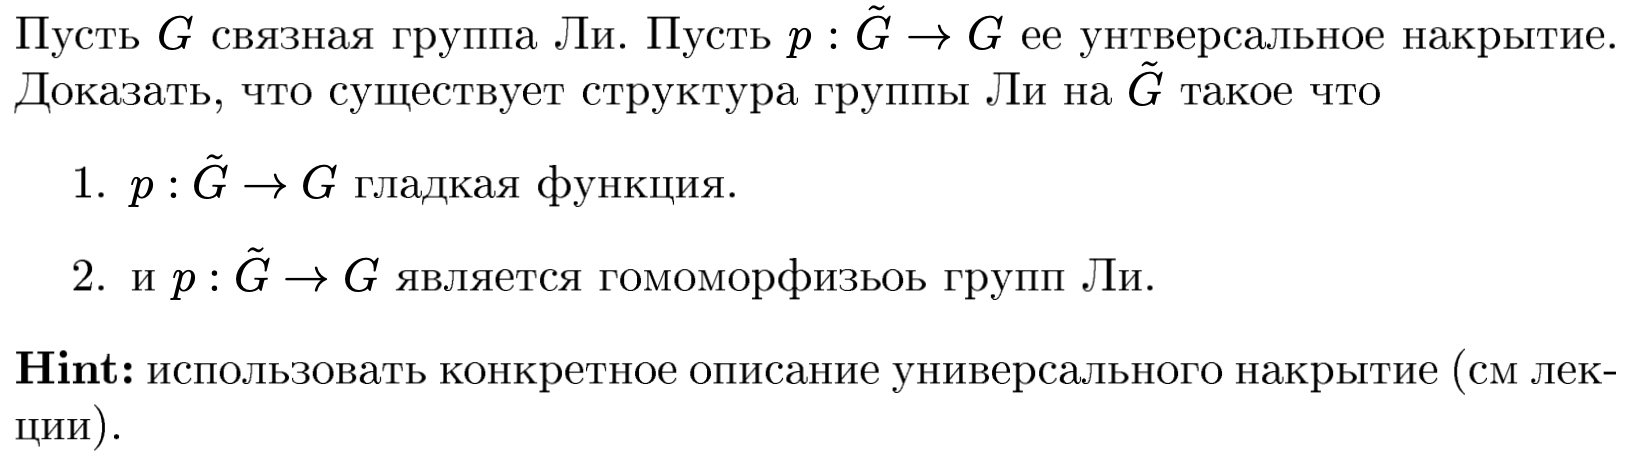
\includegraphics[width=0.4\textwidth]{photo_2.png}
\end{center}
\par Так как у нас вакуум вне металла то $\theta = \theta'$
\par Граничные условия:
\[
    E_{x1} = E_{x2}
\]
\[
    E_{x1} = E_0 \cos \theta - r E_0 \cos \theta
\]
\[
    E_{x2} = t E_0 \cos \theta
\]
\[
    \Rightarrow 1 - r = t
\]
\[
    \oint \overrightarrow{H} d \vec{l} = \frac{4 \pi}{c} \overrightarrow{I} + \frac{1}{c} \int \frac{\partial \overrightarrow{E}}{\partial t} d\overrightarrow{S}
\]
\[
     \Rightarrow E_{x2} - E_{x1} = \frac{4\pi}{c} j = \frac{4\pi}{c} \sigma E_x
\]
\[
    rot \overrightarrow{E} = -\frac{1}{c} \frac{\partial \overrightarrow{H}}{\partial t}
\]
\par У $H$ только $y$ компонента, получаем:
\[
    \frac{\partial E_z}{\partial x} - \frac{\partial E_x}{\partial z} = \frac{i \omega }{c} H_y
\]
\[
    \frac{c}{i \omega} \left[  \frac{\partial E_{z2}}{\partial x} - \frac{\partial E_{x2}}{\partial z} - \left( \frac{\partial E_{z1}}{\partial x} - \frac{\partial E_{x1}}{\partial z} \right) \right] = \frac{4\pi}{c} \sigma E_{x2}
\]
\[
    \overrightarrow{E} = E_0 \left( \cos \theta \vec{e_x} + \sin \theta \vec{e_z} \right) e^{ikx\sin \theta  + ik y\cos \theta  - i\omega t}
\]
\begin{eqnarray*}
    \frac{c}{i \omega} \left[ ik \sin \theta t E_0 \sin \theta - ik \cos \theta t E_0 \cos \theta - \left( ik \sin \theta \left( E_0 + r E_0 \right) \sin \theta - \right. \right. \\
    \left. \left. - ik \cos \theta \left( E_0 + r E_0 \right) \cos \theta \right) \right] = \frac{4\pi}{c} \sigma t E_0 \cos \theta
\end{eqnarray*}
\[
    k = \frac{\omega}{c}
\]
\[
    t \sin^2 \theta - t \cos^2 \theta - \left( \sin^2 \theta \left( 1 + r \right) + \cos^2 \theta \left( 1 - r \right) \right) = \frac{4\pi}{c} \sigma t \cos \theta
\]
\[
    r \cos 2\theta - 1 - t\cos 2\theta = \frac{4\pi}{c} \sigma t \cos \theta
\]
\begin{eqnarray*}
    \begin{cases}
        1 - r = t \\
        r \cos 2\theta - 1 - t\cos 2\theta = \frac{4\pi \sigma}{c} t \cos \theta
    \end{cases}
\end{eqnarray*}
\begin{eqnarray*}
    \begin{cases}
        1 - t = r \\
        \cos 2\theta - 1 - 2 t\cos 2\theta = \frac{4\pi \sigma}{c} t \cos \theta
    \end{cases}
\end{eqnarray*}
\begin{eqnarray*}
    \begin{cases}
        r = \frac{\cos 2\theta + \frac{4\pi \sigma}{c} \cos \theta +1 }{2\cos 2\theta + \frac{4\pi \sigma}{c} \cos \theta} \\
        r = \frac{\cos 2\theta -1 }{2\cos 2\theta + \frac{4\pi \sigma}{c} \cos \theta}
    \end{cases}
\end{eqnarray*}
\par Ответ:
\begin{eqnarray*}
    \begin{cases}
        r = \frac{\cos 2\theta + \frac{4\pi \sigma}{c} \cos \theta +1 }{2\cos 2\theta + \frac{4\pi \sigma}{c} \cos \theta} \\
        r = \frac{\cos 2\theta -1 }{2\cos 2\theta + \frac{4\pi \sigma}{c} \cos \theta}
    \end{cases}
\end{eqnarray*}
\par
\par
\end{large}
\end{document}
